\section{Condition monitoring}
All rotating machinery eventually fails because of the long-term strain on the individual parts or incorrect workmanship, installation, or operational procedures. In the end, these factors cause the equipment not to fulfill its intended functionality. Many instrumentation methods are practiced to reveal evolving faults: vibration and acoustic noise monitoring, electric supply line measurements, thermography, oil and particle analysis, ultrasonic testing, etc. Vibration signals are the preferred tool for rotating machinery monitoring \cite{mohanty_machinery_2015}. 

The defect needs to be either repaired or replaced, preferably without significant production downtime, further damage to the other attached elements, or any endangerment of the responsible personnel. The maintenance strategies are chosen according to the machine's importance as a result of its failure effect evaluation on the system. The guide to set appropriate maintenance procedures is outlined by IEC 60706-2 standard and involves reliability-centered maintenance (RCM) analysis \cite{el-thalji_predictive_2019}.

\subsection{Maintenance strategies}
There are three different approaches to maintenance across the industry: reactive, preventive, and predictive \cite{scheffer_practical_2004}. In general, the more sophisticated methods are beneficial in a high-stakes environment. The unexpected machine shutdown can have a negative economic impact on the enterprise, resulting in decreased product quality and demands spare parts be ready in the supply inventory at all times. However, in certain situations suffice to utilize a simpler maintenance program, but predictive maintenance gains interest in the Industry 4.0 to optimize assets' usage  \cite{cinar_machine_2020}.
\bigbreak

\textbf{Reactive maintenance} allows machinery to run to complete failure. This is the most inappropriate way to maintain the production line, but it is straightforward. It requires a large stock of replacement parts on-site and breakage inflict a `crisis management mode' upon the plant \cite{scheffer_practical_2004}. On-demand repairs are justified for consumer products or in the factory capable of fully and quickly replacing the halted machine with a backup. 
\bigbreak

\textbf{Preventive maintenance} is performed before any issue is detected. Maintenance occurs at regular intervals derived from a predetermined period in the calendar or expected machine running time (e.g. MTTF - Mean Time To Failure). The schedule is crucial but can result in components being replaced in good condition when further utilization is possible or too late after the machine breaks. In this case, conservative planning is usually the norm to keep machine always in perferct state and therefore more frequent intervention. \cite{mohanty_machinery_2015}.  
\bigbreak

\textbf{Predictive maintenance} known as condition-based maintanance (CbM), improves the predictability of reactive maintenance and eliminates the waste in overall resource utilization of cautious prevention. The machine downtime is scheduled after the detection of unhealthy trends in fault monitoring with sensors and troublesome components are identified. 

Measurable decrease in efectivity allows us to order necessary parts in advance and organize repairs of several machines at a convenient time. The misdetection leads to increased costs compared to previous methods and raises the expectation that faults are distinguishable among themselves~\cite{davies_handbook_2012}.

\bigbreak

\begin{figure}[h]
	\centering
	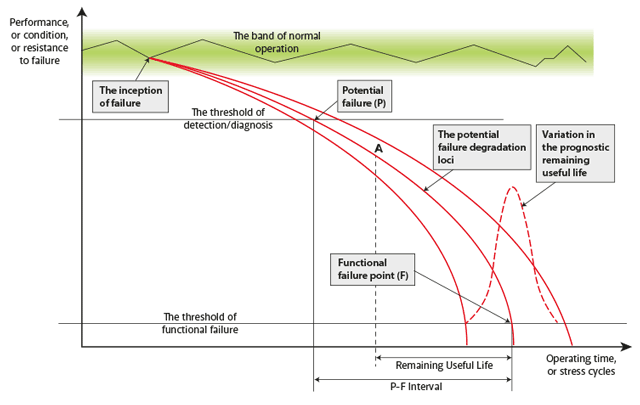
\includegraphics[width=\textwidth]{assets/P-F-Curve.png}
	\caption{P-F curve represets evolution of the asset's health \cite{jennions_integrated_2011}}
	\label{fig:p-f-curve}
\end{figure}

The P-F curve is a widespread representation of equipment degradation over time based on historical records (Fig.~\ref{fig:p-f-curve}). Corrective action should be taken between the event of potential failure (P), when the fault detection is activated, and functional failure point (F) in the P-F interval~\cite{bousdekis_enterprise_2021}.  These division points are not exactly set but have statistical distribution to them.

The Remaining Useful Life (RUL) of the specific running machine in the given instance can be merely estimated analytically, with the survival probabilities of the individual components, and based on the model of the `run-to-failure' histories and usage parameters~\cite{okoh_overview_2014}. Predictive condition monitoring aims to extend the machine lifespan to the maximum by predicting expected RUL.

\begin{figure}[h]
	\centering
	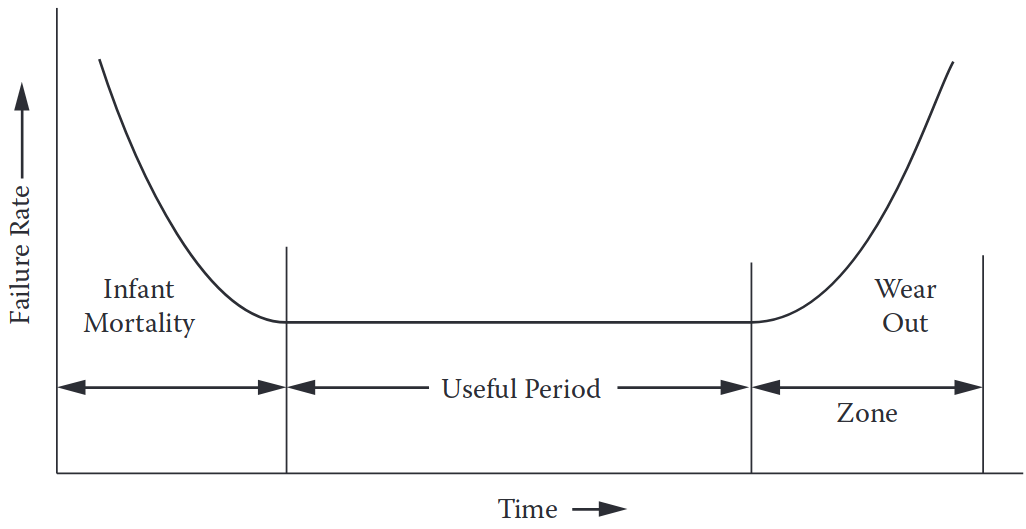
\includegraphics[width=0.8\textwidth]{assets/bath-tub-curve.png}
	\caption{Bath tub curve~\cite{mohanty_machinery_2015}}
	\label{fig:bath-tub-curve}
\end{figure}

High failure rate is present not only at the worn out stage when the parts are fatigued or corroded, but also in the early stages soon after assembly. Causes can be found in the manufacturing or material defects, inadequate installation, or improper start-up procedures. During the stable middle phase the malfunction can occur after machine excessive overload. The time plot to failure rate is known as the bath tub curve (Fig.~\ref{fig:bath-tub-curve}).

\subsection{Vibration fault types}
Mechanical problems during machinery operation bring about vibrations in the vast majority of cases. The cause of vibration comes out of the changing force in its magnitude or direction. The most emerging defects can be encompassed by explaining the deficiencies of the mechanical structure broadly categorized as \textbf{unbalance, misalignment, looseness, excentricity, and influence of the external force}~\cite{davies_handbook_2012}. 

However, rotating machine disorders do exhibit frequency signatures at various ranges in the frequency spectrum. Imbalance, misalignment, and looseness normally appear at frequencies up to 300 Hz. These low-frequency faults are associated with the movement of the shaft and primarily coincide with revolution speed and its harmonics. Bearing and gearbox defects in the late stages of development, show up in the range between 300 Hz to 1 kHz. Higher frequencies measured traditionally to a limit of 10 kHz help notice the flaw of bearings even sooner~\cite{torres_automatic_2022}.


\begin{itemize}
\item predominant frequency
\item synchronous frequency
\item subsynchronous frequency
\item fundamental frequency
\item harmonic frequency
\item subharmonic frequency
\end{itemize}
% p.294 Davies

\cite{scheffer_practical_2004} p.98 - 141

\cite{davies_handbook_2012} p.282
% Automatic Anomaly Detection in Vibration Analysis Based on Machine Learning Algorithms
\cite{torres_automatic_2022}
% Vibration Guide
\cite{noauthor_vibration_2000}
% The experimental application of popular machine learning algorithms on predictive maintenance and the design of IIoT based condition monitoring system
\cite{cakir_experimental_2021}
% Technická diagnostika
\cite{ziaran_technicka_2013}
 
%TODO
Why monitor with vibrations,
- Resonance frequencies of each part - machine must run at speeds not aligned with resonance frequencies - Campbell diagram - task for mechanical engineers
- Faults - reasons and frequency content

% Describe by frequency responses and assign them possibale faults instead

\begin{itemize}
\itemsep0pt
\item Synchrounous response - based on RPM
\item Mass unbalance
\item Misalignment
\item Eccentricity
\item Bent or bow shaft
\item Cracked shaft
\item Rotor rubs - friction
\item Looseness
\item Auxiliery mechanical systems: Gearbox, Bearings, Belt 
\end{itemize}

% Bandsaws
% Vibration of bandsaws
\cite{lengoc_vibration_1990}
% Study on Online Detection and Fault Diagnosis of Band Saw Equipment
\cite{chen_study_2014}

\subsection{Technical standards}
Vibration-based condition monitoring practices adopted in the factory's predictive maintenance management must comply with normative guidelines formalized in ISO international standards. The standards are concerned with each step in the process that originates with transducer placements and data acquisition. They prescribe conventions for setting fault severity levels and provide empirically observed vibration characteristics of common defects. Two relevant standards for IoT diagnostics systems are \emph{ISO 20816} (updated from ISO 10816) and \emph{ISO 13373}.
\bigbreak

\textbf{ISO 20816-1:2016} establishes the approach to vibration measurement and evaluation on non-rotating housing of machinery parts~\cite{noauthor_iso_2016}. The measurement units are agreed upon for kinematic quantities of vibrations. Acceleration is to be measured in meters per second squared ($m/s^2$), velocity in millimeters per second ($mm/s$), and displacement in micrometers ($\mu m$). It is customary to evaluate broad-band vibration velocity in terms of root mean square value (RMS), as it has a relation to its signal energy. No simple direct relationship is expressible among these quantities, except in stationary signals.

The vibration severity is the maximum magnitude value measured in two radial directions (horizontal, and vertical) or supplemented with a third direction along the shaft in the axial axis. Multiple measurement locations, i.e. on several bearings or couplings, should be assessed independently. 

Criteria introduced to judge vibration severity are its absolute vibration magnitude, change in the magnitude vector, and rate of change. In terms of maximal magnitudes the machines of varied sizes are split into four severity zones defined in the chart ~(Tab.~\ref{tab:iso20816-vibration-severity}). The table values serve as guidelines towards realistic requirements between machinemanufacturers and customers.

\begin{table}[h]
\renewcommand{\arraystretch}{1.2}
\begin{adjustbox}{width=\columnwidth,center}
\begin{tabular}{|c|c|c|c|c|}
\hline
\textbf{\begin{tabular}[c]{@{}c@{}}Vibration velocity\\ RMS {[}mm/s{]}\end{tabular}} & \textbf{\begin{tabular}[c]{@{}c@{}}Class I\\ Small machines\end{tabular}} & \textbf{\begin{tabular}[c]{@{}c@{}}Class II\\ Medium machines\end{tabular}} & \textbf{\begin{tabular}[c]{@{}c@{}}Class III\\ Large machines\\ Rigid supports\end{tabular}} & \textbf{\begin{tabular}[c]{@{}c@{}}Class IV\\ Large machines\\ Flexible support\end{tabular}} \\ \hline
0.28                                                                                 & \cellcolor[HTML]{9AFF99}                                                  & \cellcolor[HTML]{9AFF99}                                                    & \cellcolor[HTML]{9AFF99}                                                                     & \cellcolor[HTML]{9AFF99}                                                                      \\ \cline{1-1}
0.45                                                                                 & \cellcolor[HTML]{9AFF99}                                                  & \cellcolor[HTML]{9AFF99}                                                    & \cellcolor[HTML]{9AFF99}                                                                     & \cellcolor[HTML]{9AFF99}                                                                      \\ \cline{1-1}
0.71                                                                                 & \multirow{-3}{*}{\cellcolor[HTML]{9AFF99}\textbf{Good (A)}}               & \cellcolor[HTML]{9AFF99}                                                    & \cellcolor[HTML]{9AFF99}                                                                     & \cellcolor[HTML]{9AFF99}                                                                      \\ \cline{1-2}
1.12                                                                                 & \cellcolor[HTML]{FFFC9E}                                                  & \multirow{-4}{*}{\cellcolor[HTML]{9AFF99}\textbf{Good (A)}}                 & \cellcolor[HTML]{9AFF99}                                                                     & \cellcolor[HTML]{9AFF99}                                                                      \\ \cline{1-1} \cline{3-3}
1.8                                                                                  & \multirow{-2}{*}{\cellcolor[HTML]{FFFC9E}\textbf{Satisfactory (B)}}       & \cellcolor[HTML]{FFFC9E}                                                    & \multirow{-5}{*}{\cellcolor[HTML]{9AFF99}\textbf{Good (A)}}                                  & \cellcolor[HTML]{9AFF99}                                                                      \\ \cline{1-2} \cline{4-4}
2.8                                                                                  & \cellcolor[HTML]{F8A102}                                                  & \multirow{-2}{*}{\cellcolor[HTML]{FFFC9E}\textbf{Satisfactory (B)}}         & \cellcolor[HTML]{FFFC9E}                                                                     & \multirow{-6}{*}{\cellcolor[HTML]{9AFF99}\textbf{Good (A)}}                                   \\ \cline{1-1} \cline{3-3} \cline{5-5} 
4.5                                                                                  & \multirow{-2}{*}{\cellcolor[HTML]{F8A102}\textbf{Unsatisfactory (C)}}     & \cellcolor[HTML]{F8A102}                                                    & \multirow{-2}{*}{\cellcolor[HTML]{FFFC9E}\textbf{Satisfactory (B)}}                          & \cellcolor[HTML]{FFFC9E}                                                                      \\ \cline{1-2} \cline{4-4}
7.1                                                                                  & \cellcolor[HTML]{FD6864}                                                  & \multirow{-2}{*}{\cellcolor[HTML]{F8A102}\textbf{Unsatisfactory (C)}}       & \cellcolor[HTML]{F8A102}                                                                     & \multirow{-2}{*}{\cellcolor[HTML]{FFFC9E}\textbf{Satisfactory (B)}}                           \\ \cline{1-1} \cline{3-3} \cline{5-5} 
11.2                                                                                 & \cellcolor[HTML]{FD6864}                                                  & \cellcolor[HTML]{FD6864}                                                    & \multirow{-2}{*}{\cellcolor[HTML]{F8A102}\textbf{Unsatisfactory (C)}}                        & \cellcolor[HTML]{F8A102}                                                                      \\ \cline{1-1} \cline{4-4}
18                                                                                   & \cellcolor[HTML]{FD6864}                                                  & \cellcolor[HTML]{FD6864}                                                    & \cellcolor[HTML]{FD6864}                                                                     & \multirow{-2}{*}{\cellcolor[HTML]{F8A102}\textbf{Unsatisfactory (C)}}                         \\ \cline{1-1} \cline{5-5} 
28                                                                                   & \cellcolor[HTML]{FD6864}                                                  & \cellcolor[HTML]{FD6864}                                                    & \cellcolor[HTML]{FD6864}                                                                     & \cellcolor[HTML]{FD6864}                                                                      \\ \cline{1-1}
45                                                                                   & \multirow{-5}{*}{\cellcolor[HTML]{FD6864}\textbf{Unacceptable (D)}}       & \multirow{-4}{*}{\cellcolor[HTML]{FD6864}\textbf{Unacceptable (D)}}         & \multirow{-3}{*}{\cellcolor[HTML]{FD6864}\textbf{Unacceptable (D)}}                          & \multirow{-2}{*}{\cellcolor[HTML]{FD6864}\textbf{Unacceptable (D)}}                           \\ \hline
\end{tabular}
\end{adjustbox}
\caption{ISO 20816 vibration serverity chart \cite{noauthor_iso_2016}}
\label{tab:iso20816-vibration-severity}
\end{table}

\emph{Zone A} is reserved for newly commissioned machines. \emph{Zone B} signifies suitability for long-term operation. In \emph{zone C} is the machine deemed in unsatisfactory condition and corrective action should be taken soon. Finally, in zone D vibrations can cause damage to the machine. The span of acceptable values differs on machine class from I through to IV with an output power of 15 kW (class I), 75 kW (class II), 10 MW (class III), or greater.

The operational limits in the form of \emph{alarms} and \emph{trips} are usually established on the zone boundaries or close to them. Alarms are placed between zones B and C and provide a warning about reaching the threshold significant for noticeable change. Trips in between zones C and D urge immediate action or machine shut down.

\textbf{ISO 13373-1:2002} delves into further nuances of vibration monitoring and expands on procedures outlined in the vocabulary of ISO 20186. According to the standard, the data collection operates in continuous or periodic observation modes which follow an event or intervals. Both designs can be permanently mounted, but in continuous, collection `multiplexing rate is sufficiently rapid so there is no significant data or trends lost'~\cite{noauthor_iso_2002}.  When channels are scanned successively with gaps between data points the system is known as `scanning'. 

Measurement of vibrations should be accompanied by a description of the machine and its operating conditions. The machine description includes the machine identifier and its type, power source, rated rotation speed and power, configuration (shaft or belt driven), and machine support. Measurement parameters such as timestamp, transducer type, sensor location and orientation in MIMOSA code, measurement units and units qualifier (p-p, RMS), and other processing options (filters, number of averages, etc.) are to be recorded alongside the measurement value itself~\cite{noauthor_iso_2002}.
  
The transducer of choice for condition monitoring is the accelerometer which can provide the acceleration value of the body and velocity after signal integration. However, standard cautions against double integrating for displacement. The recommended frequency range for an accelerometer is 0.1 Hz to 30 kHz. The choice of transducer mount significantly lowers its resonance frequency which is least influenced by stud mount and stiff cement mount. The resonance is reduced to around 8 kHz with the use of soft epoxy or permanent magnet.

\begin{figure}[h]
	\centering
	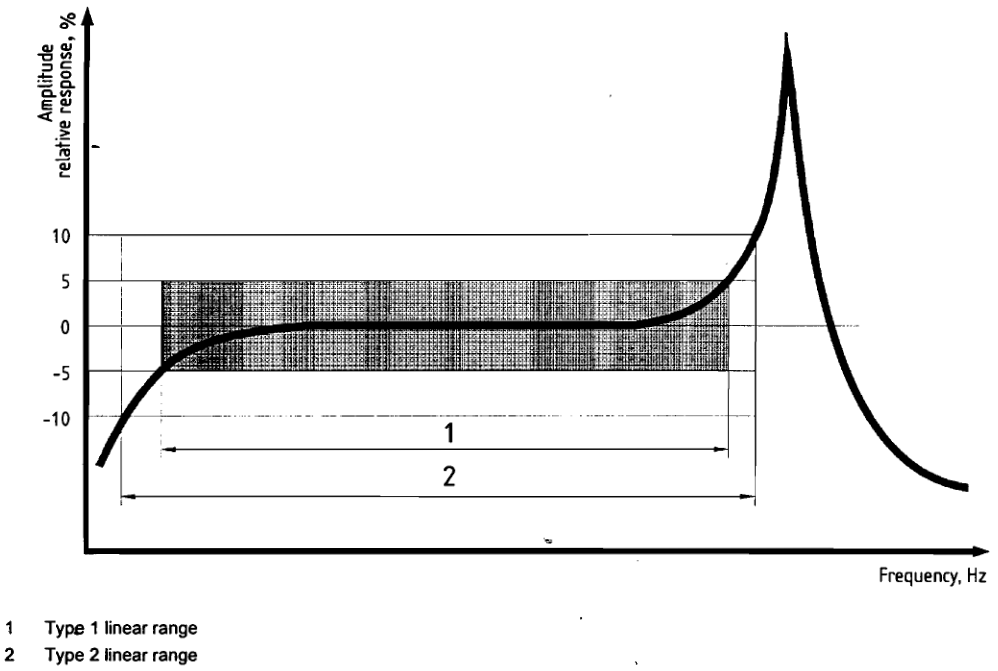
\includegraphics[width=0.8\textwidth]{assets/transducer-response.png}
	\caption{The transducer linear response and resonance in tolerance intervals~\cite{noauthor_iso_2002}}
	\label{fig:tranducer-response}
\end{figure}

Broadband measurement requires `frequency ranges of 0.2 times the lowest rotational frequency to the highest frequency of interest' \cite{noauthor_iso_2002}, not exceeding 10 kHz, with RMS velocity 0.1 - 100 mm/s. Bearings and gears diagnosis may push the upper-frequency limit even higher. The tolerances of amplitude and frequency calibrations fall into two types with allowable tolerances of $\pm 5 \%$ or $\pm 10 \%$ (Fig.~\ref{fig:tranducer-response}). 



 
% Different under load 
% Baseline measurement - what are those p.28
% Monitoring programme p.12 (vibrations differ under load)
% Later: Potencial causes for faults (p. 45) - use in vibration fault types

\begin{enumerate}
\itemsep0pt
\item Review machinery history and establish failure modes.
\item When vibration monitoring is not applicable check for other condition monitoring techniques or use preventive maintance routine.
\item Select monitoring points
\item Take preliminary vibration measurements
\item Select vibration monitoring techniques: broadband, frequency analysis or special techniques. Set parameters of measurements units.
\item Take baseline measurements
\item Change levels that would warrant investigation
\item Carry out routine condition monitoring
\item If alarm was exceeded notify approriate personnel, review data and trends, perform diagnostic evaluation, repair as necessary. In case new baseline is needed continue in step of taking baseline measurements.
\item Shut down machine when trip level is exceeded. Than proceed same as after alarm trigger.
\end{enumerate}

\newpage

 
